% !TEX encoding = UTF-8 Unicode
 
\documentclass[11pt, a4paper]{article}
 
\usepackage[utf8]{inputenc}
\usepackage[pdftex]{graphicx}
%\usepackage{graphicx}
\usepackage{amsmath}
 
\addtolength{\textwidth}{1.75in}
\addtolength{\oddsidemargin}{-.875in}
\addtolength{\evensidemargin}{-.875in}
\addtolength{\topmargin}{-70pt}
\addtolength{\textheight}{70pt}
  
\begin{document}
%\begin{center}
\begin{center}
{\noindent \huge \bf Relational Reasoning Model }\\
\end{center}
 
We present a probabilistic model for Caren and Alison's Relational Reasoning experiment and the results obtained with it.
 
\section*{The Model}
We use a hierarchical model with three levels: the \emph{theory} level, the \emph{hypotheses} level, and the \emph{data} level. At the \emph{theory} level, there is a single variable $t$ indexing the different theories. The \emph{hypotheses} level has a richer structure, amounting for the hypotheses corresponding to the different theories and number of blocks needed simultaneously. Finally, at the \emph{data} level, we describe actions (placing an arbitrary number of blocks on the machine) together with the results (either the machine going or not), and the bold notation describes many single datapoints. We allow for blocks of an arbitrary number of shapes $n_s$ to be present.
 
 
\subsection*{The \emph{theory} level}
We consider three types of theory: $t=0$, in which individual blocks activate the machine, $t=1$, in which two blocks of equal shape are needed to activate the machine, and $t=2$, in which two blocks of different shape activate the machine. 
 
The prior probabilities for these theories are indexed by parameters $\alpha$ and $\beta$ as follows:
\begin{equation}
\begin{split}
p(t=0)&=1-\alpha-\beta\\
p(t=1)&=\alpha\\
p(t=2)&=\beta.
\end{split} 
\end{equation}
 
\subsection*{The \emph{hypotheses} level}
Hypotheses here are specific combinations of shapes that one thinks activate the machines. Examples of hypotheses are ``a single triangular shape will activate the machine'', or ``the combination of two triangular shapes or two circular shapes will activate the machine''. They are indexed by a triad $h=(h_0,h_1,h_2)$, where $h_0$ indexes which type of theory the hypothesis corresponds to, that is, $h_0=0$ tells us that $h$ corresponds to an individual-block theory, $h_0=1$ that it corresponds to the equal shape theory, and $h_0=2$ to the different shape one.
 
$h_1$ labels the number of different blocks (or equal/different pairs thereof) that activate the machine according to the hypothesis. For instance, $h_1=1$ means that a single shape activates the machine in the case $h_0=0$ (say triangles, but not squares or circles), and that a single pair of equal shapes activates the machine in the case $h_0=1$ (say two squares but not two circles, etc). The special case $h_1=0$ means that no shape can activate the machine. $h_1$ ranges between 0 and $n_s$ for $h_0=0$ and between 1 and $n_s$ for $h_0=1$ (since we already incorporated the special no activation case to the first theory). For $h_0=2$, $h_1$ ranges between 1 and $n_2 \choose 2$.
 
Finally, $h_2$ is the remaining label indexing the different possibilities for given $h_0$ and $h_1$, and its range varies with the values of $h_0$ and $h_1$. In general, we have $h_2\in\{0, \ldots, {\textrm{range}(h_1) \choose h_1 }\}$, where $\textrm{range}(h_1)$ depends on the value of $h_0$ as detailed above. For instance, having $h_0=0$ (individual blocks) and $h_1=1$ (single shape), gives us $h_2\in\{0, \ldots, n_s-1\}$, that is, there are $n_s$ different shapes that could be responsible for activating the machine, each corresponding to a different hypothesis. 
 
\subsection*{The theory-hypothesis likelihood}
The theory-hypothesis likelihood is defined as:
\begin{equation}
p(h|t) \propto
\begin{cases}
\gamma^{h_1} & \mbox{if } t=h_0 \\ 
0 & \mbox{otherwise}.
\end{cases}
\end{equation}
where $\gamma$ is a parameter in the range $[0,1]$ and the distribution is normalized for each value of $t$. This equation penalizes hypotheses with a big number of blocks (or pairs of blocks).
 
\subsection*{The \emph{data} level and the data-hypothesis likelihood}
Single datapoints are (\emph{action}, \emph{result}) pairs, where \emph{action} is either bringing a single or a pair of blocks in contact with the machine and \emph{result} $\in\{ \textrm{True, False} \}$, indicates whether the machine lit up or not. The whole sequence of play $\textbf d$ is a collection of datapoints $d$. The different datapoints in the sequence are conditionally independent given the hypothesis, such that we need only look at the data-hypothesis likelihood for a single datapoint $d$:
\begin{equation}
p(d|h)= 
\begin{cases} 
1  & \textrm{if $d$ is compatible with  $h$} \\
\epsilon &  \textrm{if it is not},
\end{cases}
\end{equation}
where $\epsilon$ is a free noise parameter. Compatibility here means that the block in $d$ satisfies the criteria specified by $h$ for the machine to activate, if the state of the machine in $d$ is active, or that the block fails to satisfy the criteria in $h$, and the state of the machine is inactive. Although this distribution is also not normalized, we don't need to normalize it explicitly, since the constant will cancel in our further computations (weak sampling). 
 
\subsection*{Full joint distribution}
The full joint distribution then simply factorizes as:
\begin{equation}
p(\textbf d,h,t)=p(\textbf d |h)p(h|t)p(t),
\end{equation}
keeping in mind that $p(\textbf d |h)=\prod_i p(d_i |h)$, where $\textbf d$ is a sequence of individual datapoints $d_i$.
 
\subsection*{Predictive probability}
We are interested in predicting whether a new choice of block (shape) will activate the machine. For this, we need to compute the probability of a new datapoint given a history of previously observed data. Calling $d_n$ the new (predicted) datapoint, and $\textbf d_o$ the previously observed sequence, we have:
\begin{equation}
\begin{split}
p(d_n|\textbf d_o)&=\sum_h p(d_n|h)p(h|\textbf d_o)\\
&=\sum_{h,t} p(d_n|h) p(h|\textbf d_o, t) p(t|\textbf d_o)\\
&=\sum_{h,t} p(d_n|h) \frac{p(\textbf d_o| h, t) p(h|t)}{p(\textbf d_o|t)} p(t|\textbf d_o)\\
&=\sum_{h,t} p(d_n|h) p(\textbf d_o| h) p(h|t)\frac{p(t)}{p(\textbf d_o)}.
\end{split}
\end{equation}
Here, in going from the third to the last line, we used the fact that, conditioned on hypotheses, the data are independent of the theory. Finally, we need an expression for $p(\textbf d_o)$:
\begin{equation}
p(\textbf d_o)=\sum_{h,t} p(\textbf d_o|h) p(h|t) p(t).
\end{equation}
 
\subsection*{Choice}
Since we want to model the children's choices, we still need to include in our model a recipe for the choice. Children are offered two options of action in the experiment, which we denote by $a_1$ and $a_2$. We model the probability of choosing action $a_1$ as:
\begin{equation}
p_{choice}(a_1)=\frac{p(\textrm{active}|a_1,\textbf d_o)}{p(\textrm{active}|a_1,\textbf d_o)+p(\textrm{active}|a_2,\textbf d_o)},
\end{equation} 
where again $\textbf d_o$ is the previously observed data, and we compute the probability of activation given an action as:
\begin{equation}
p(\textrm{active}|a,\textbf d_o)= p(d^{\textrm{active}}_n|\textbf d_o),
\end{equation}
where $d^{\textrm{active}}_n$ is a single datapoint formed by joining action $a$ with an \emph{active} (or True) result.
 
 
\section*{Results}
\subsection*{Experiment data}
For the moment, we focus on reproducing the average number of correct choices in the two \emph{same}/\emph{different} conditions for Experiment 1 (no manipulation) and Experiment 2 (negative evidence for single object given). Because the complexity of the model grows exponentially with the number of available shapes, we simplify the treatment by presenting a single piece of evidence of each kind, so that in the \emph{same} condition the model sees a pair of identical shapes activating the machine and a pair of different shapes not activating it, and viceversa for the \emph{different} condition. The actual children see two independent instances of each, but attempting to include this renders the model intractable. In modeling Experiment 2, we add to this the evidence of single block non-activations, identical in both conditions, prior to seeing the conjoint evidence.
 
The actual success probabilities from the experiment are:
\begin{equation}
\begin{split}
p^{E1,same}_{corr}&=0.46,\\
p^{E1,diff}_{corr}&=0.43,\\
p^{E2,same}_{corr}&=0.79,\\
p^{E2,diff}_{corr}&=0.5.
\end{split}
\end{equation}
 
 
\subsection*{Manual minimization}
Our model has four free parameters that we need to choose: $\alpha$, $\beta$, $\gamma$ and $\epsilon$. We vary these parameters by hand to minimize the sum of the squared differences of the four target probabilities, model minus data. The range of the parameters chosen is:
\begin{equation}
\begin{split}
\alpha&\in\{0.01, 0.05, 0.2, 0.33, 0.5, 0.9\},\\
\beta&\in\{0.01, 0.05, 0.2, 0.33, 0.5, 0.9\},\\
\gamma&\in\{0.01, 0.1, 0.5, 0.9, 0.99\},\\
\epsilon&\in\{0.001, 0.01, 0.05, 0.1, 0.25\}.
\end{split}
\end{equation}
Parameters $\alpha$ and $\beta$ were always chosen such that $\alpha+\beta\leq1$. The choice among these values that minimizes the error is:
\begin{equation}
(\alpha,\beta,\gamma,\epsilon)=(0.33,0.01,0.99,0.25),
\end{equation}
and the probabilities they yield are:
\begin{equation}
\begin{split}
p^{M1,same}_{corr}&=0.55,\\
p^{M1,diff}_{corr}&=0.54,\\
p^{M2,same}_{corr}&=0.65,\\
p^{M2,diff}_{corr}&=0.51,
\end{split}
\end{equation}
where we substituted $M$ for $E$ to indicate that these are model results. This shows that, although the numbers are not exactly the same, the general effect observed in the experiment can be recovered by the model. In particular, we see an increase in the probability of a correct choice for the second experiment only in the $same$ condition, which is the crucial effect in the study. 
 
A note is in place however regarding the parameter values, since three of them $\beta$, $\gamma$ and $\epsilon$ are on the boundary of their allowed region. Although one can extend this region in an attempt to improve the match between model and data even further, we see that the values are already too extreme. In particular, a value of $\epsilon=0.25$ seems like an unreasonable amount of noise. On the good side, however, 
we find that with a less extreme choice of parameters as $(\alpha,\beta,\gamma,\epsilon)=(0.3,0.02,0.9,0.05)$, we can still coarsely find the desired effect, finding correct-choice probabilities of $(0.60, 0.59, 0.87, 0.67)$ (in the same order as above). 
 
 
 
\subsection*{Automatic minimization}
Running an automatic optimization over the range of the parameters taking into account the probability constraints we reach similar values, namely: $(\alpha,\beta,\gamma,\epsilon)=(0.29,0,1,0.15)$, with correct choice probabilities of $(0.56, 0.56, 0.73, 0.53)$. This again shows the main effect and is slightly closer in value to the experimental data. 
 
 
\section*{Model Variations 1: Another Theory}
Given the results above, and their stability against changes in $\epsilon$ and $\gamma$, we introduce a variation of the model where these two parameters are fixed to $\epsilon=0.1$ and $\gamma=1$. This amounts to a moderate amount of noise and no penalization for hypotheses with big numbers of block combinations. Further, we include a new alternative at the level of theories that describes the possibility that any two blocks activate the machine (no matter whether they are similar or different). With this, we have the following changes in the model description.

\subsection*{The \emph{theory} level}
The new theory prior is as follows:
\begin{equation}
\begin{split}
p(t=0)&=1-\alpha-\beta-\delta\\
p(t=1)&=\alpha\\
p(t=2)&=\beta\\
p(t=3)&=\delta.
\end{split} 
\end{equation}
 
\subsection*{The theory-hypothesis likelihood}
The theory-hypothesis likelihood is now defined as:
\begin{equation}
p(h|t) \propto
\begin{cases}
1 & \mbox{if } t=h_0 \textrm{ or } (t=3 \textrm{ and } h_0\in{1,2}) \\ 
0 & \mbox{otherwise}.
\end{cases}
\end{equation}
This equation states the fact that the new `any two blocks' ($t=3$) theory supports hypotheses both of the \emph{similar} ($h_0=1$) or the \emph{different} ($h_0=2$) kinds. As before, normalization of this distribution is per theory class.
 
Since we already had a description of all kinds of pairs of blocks at the hypothesis level (split in similar and different), the rest of the model components remain unchanged. 
 
\subsection*{Model Optimization}
We ran a manual optimization over the grid:
\begin{equation}
\begin{split}
\alpha&\in\{0.01, 0.1, 0.33, 0.5, 0.66, 0.9, 0.99\},\\
\beta&\in\{0.01, 0.1, 0.33, 0.5, 0.66, 0.9, 0.99\},\\
\delta&\in\{0.01, 0.1, 0.33, 0.5, 0.66, 0.9, 0.99\}.
\end{split}
\end{equation}
The parameter values that minimize the square distance to the experimental data are $(\alpha, \beta, \delta)=(0.33,0.01,0.01)$, corresponding to correct probabilities of $(0.60, 0.57, 0.80, 0.54)$. The result is similar to what we had above: we observe the main effect, with partial quantitative match. We see that adding a theory does not improve the model fit, as the new possibility is discarded in the fit ($\delta=0.01$). 
 
\subsection*{Goodness of Fit}
Fixing $\delta=0$, we show how well the model fits the data for different values of $\alpha$ and $\beta$. The results are plotted in Fig.~\ref{fig:GoF}.
 
\begin{figure}[ht]
\centering
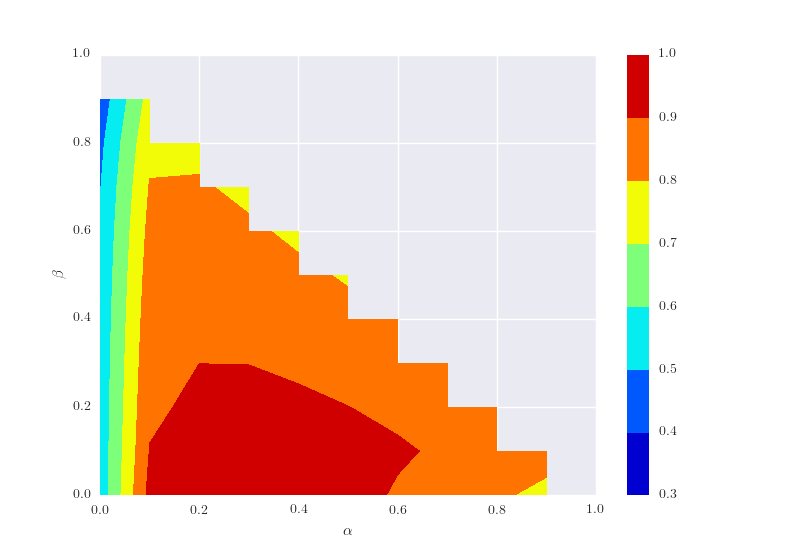
\includegraphics[width=12cm]{Figures/GoF.png}
\caption{Goodness of fit measured as 1 minus the squared distance between the vectors of correct choice probabilities, model and data. Warmer colors indicate better fit. The grey region is outside the probability simplex.}
\label{fig:GoF}
\end{figure}
 
 
 
\section*{Model Variations 2: $\alpha=\beta$}
In this section we explore a further variation of the model, returning to the original with no $\delta$ (or, equivalently, $\delta=0$), and setting $\alpha=\beta$, which leaves us with a single parameter (the other parameters are fixed to $\gamma=1$ and $\epsilon=0.1$). The model equations are the same as in the original case, keeping in mind the constraint $\alpha=\beta$. In figure~\ref{fig:GoF1} we show the goodness of fit computed as 1 minus the squared distance between the vectors of choice probabilities, model and data, as a function of $\alpha$.
\begin{figure}[ht]
\centering
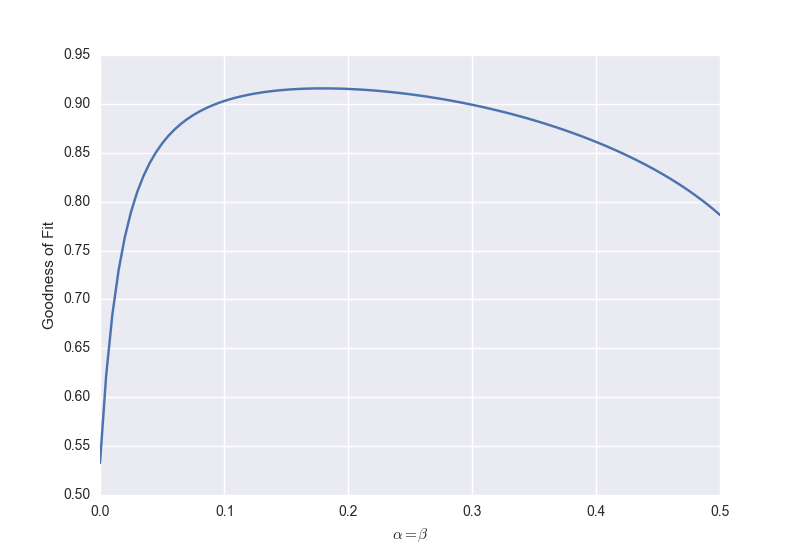
\includegraphics[width=12cm]{Figures/GoF_alpha.png}
\caption{Goodness of fit for the single parameter model.}
\label{fig:GoF1}
\end{figure} 

We performed numerical optimization over this parameter, and found that the model's predictions most closely match the experimental data at $\alpha=\beta=0.1798$, yielding correct probabilities of $(0.53, 0.60, 0.72, 0.73)$. Comparing with the data, we see that the characteristic pattern is lost. We note however that this is not due to fixing $\alpha=\beta$ but only to parameter optimization. We can recover the pattern for different values of the parameter: setting $\alpha=\beta=0.33$ yields for instance $(0.65, 0.62, 0.77, 0.71)$, which recovers the pattern in the experiment albeit with a bigger overall discrepancy in the actual numerical values. 

Finally, if we allow for a variation in the amount of noise $\epsilon$, we find through numerical optimization the minimizing values $\alpha=\beta=0.32$, $\epsilon=0.24$, which yield correct probabilities of $(0.56, 0.57, 0.62, 0.58)$. Here one can see the pattern emerge again for the optimal parameters, though very washed out and requiring a big amount of noise.  


 
\end{document}

